\documentclass[a4paper,12pt]{article} % тип документа
\usepackage[margin=1in]{geometry} % Поля

%  Русский язык
\usepackage[warn]{mathtext}
\usepackage[T2A]{fontenc}			% кодировка
\usepackage[utf8]{inputenc}			% кодировка исходного текста
\usepackage[english,russian]{babel}	% локализация и переносы
% Математика
\usepackage{amsmath,amsfonts,amssymb,amsthm,mathtools} 
\usepackage{wasysym}
%%%
\usepackage{graphicx}

\usepackage{gensymb} % знак градуса \degree

%%%% Римские цифры
\renewcommand{\thesection}{\Roman{section}.} 
\renewcommand{\thesubsection}{\roman{subsection}.}


\begin{document}
%титул
\hrule 	
\medskip
\begin{raggedright}
{\large \textbf{Отчёт по работе 2.4.1}}
\\
\medskip
{\Large Определение теплоты испарения жидкости} 
\\
\medskip
{\large Карташов Константин Б04-005}
\medskip
\hrule
\medskip
\end{raggedright}


\section{Аннотация}

\paragraph{Цель работы:}
\begin{enumerate}
\itemsep0em

\item Измерение давления насыщенного пара жидкости при разной температуре.
\item Вычисление по полученным данным теплоты испарения с помощью уравнения Клапейрона-Клаузиуса.
\end{enumerate}

\paragraph{В работе используются:}
\begin{itemize}
\itemsep0em
\renewcommand{\labelitemi}{$\triangleright$}

\item Термостат
\item Герметический сосуд, заполненный исследуемой жидкостью
\item Отсчётный микроскоп

\end{itemize}

\medskip\hrule\medskip

\section{Теоретическая часть}

\subsection{Необходимые знания для проведения эксперимента}

\paragraph{Явление испарения.}
Испарением называется переход вещества из жидкого состояние в газообразное. Оно происходит на свободной поверхности жидкости, при этом молекулы имеющие достаточную кинетическую энергию для совершения работы против внешнего давления $P$ переходят в пар. Это приводит к обеднению жидкости молекулами с высокой энергией, то есть к её охлаждению. Чтобы жидкость не остывала к ней нужно подводить тепло. Количество теплоты, необходимое для изотермического испарения одного моля жидкости при внешнем давлении, равном упругости её насыщенных паров, называется молярной теплотой испарения (парообразования).

\paragraph{Измерение теплоты парообразования.}
Измерение теплоты испарения при помощи калориметра является неточным из-за неконтролируемых потерь тепла. Поэтому для нахождения теплоты парообразования в этой работе будет использоваться метод основанный на формуле Клапейрона-Клаузиуса:

\begin{equation}
\frac{dP}{dT} = \frac{L}{T \left( V_2 - V_1 \right)}. \label{eq:c-c}
\end{equation}

\noindent Здесь $P$ - давление насыщенного газа, $T$ - температура жидкости и газа, $L$ - теплота испарения жидкости, $V_2$ - объём пара, $V_1$ - объём жидкости.

В условиях проведения эксперимента величиной $V_1$ в \eqref{eq:c-c} можно пренебречь, тогда $V_2 = V$. Также использование в качестве уравнения состояние уравнения Клапейрона будет давать ошибку менее 3\%, поэтому будет считать:

\begin{equation}
V = \frac{RT}{P} \label{eq:clap}
\end{equation}

Подставляя \eqref{eq:clap} в \eqref{eq:c-c}, пренебрегая $V_1$ и разрешая уравнение относительно $L$ получим:

\begin{equation}
L = \frac{RT^2}{P} \frac{dP}{dT} = - R \frac{d \left( \ln{P} \right)}{d \left( 1/T \right)} \label{eq:capacity}
\end{equation}

\noindent Эта формула является окончательной и будет использоваться в расчётах для нахождения $L$.

\subsection{Контрольные вопросы}

\paragraph{Вопрос 1:}
В справочниках приводится теплота испарения, измеренная при давлении 760 мм рт. ст. Совпадает ли эта величина с измеренной вами на опыте? Какая из них больше? Оцените разницу между ними.\\

Полученные в ходе эксперимента данные получились отличными от табличных. Полученное значение $L_2 = 45.2 \pm 0.7 \; \frac{\text{кДж}}{\text{моль}}$ больше табличного $L_2 = 40.68 \; \frac{\text{кДж}}{\text{моль}}$ на 10--13\%.

\paragraph{Вопрос 2:}
Укажите, исходя из теоретических соображений, в какую сторону должна меняться теплота испарения с увеличением температуры.\\

Удельная теплота парообразования уменьшается с ростом давления, так как состояние жидкости приближается к критическому, в котором фазовый переход происходит без затрат энергии. Критическое состояние происходит при высоком давлении и температуре.

\medskip\hrule\medskip

\section{Экспериментальная часть}

\subsection{Устройство экспериментальной установки}


\begin{figure}[h] % EXPERIMENTAL SETUP
\begin{center}
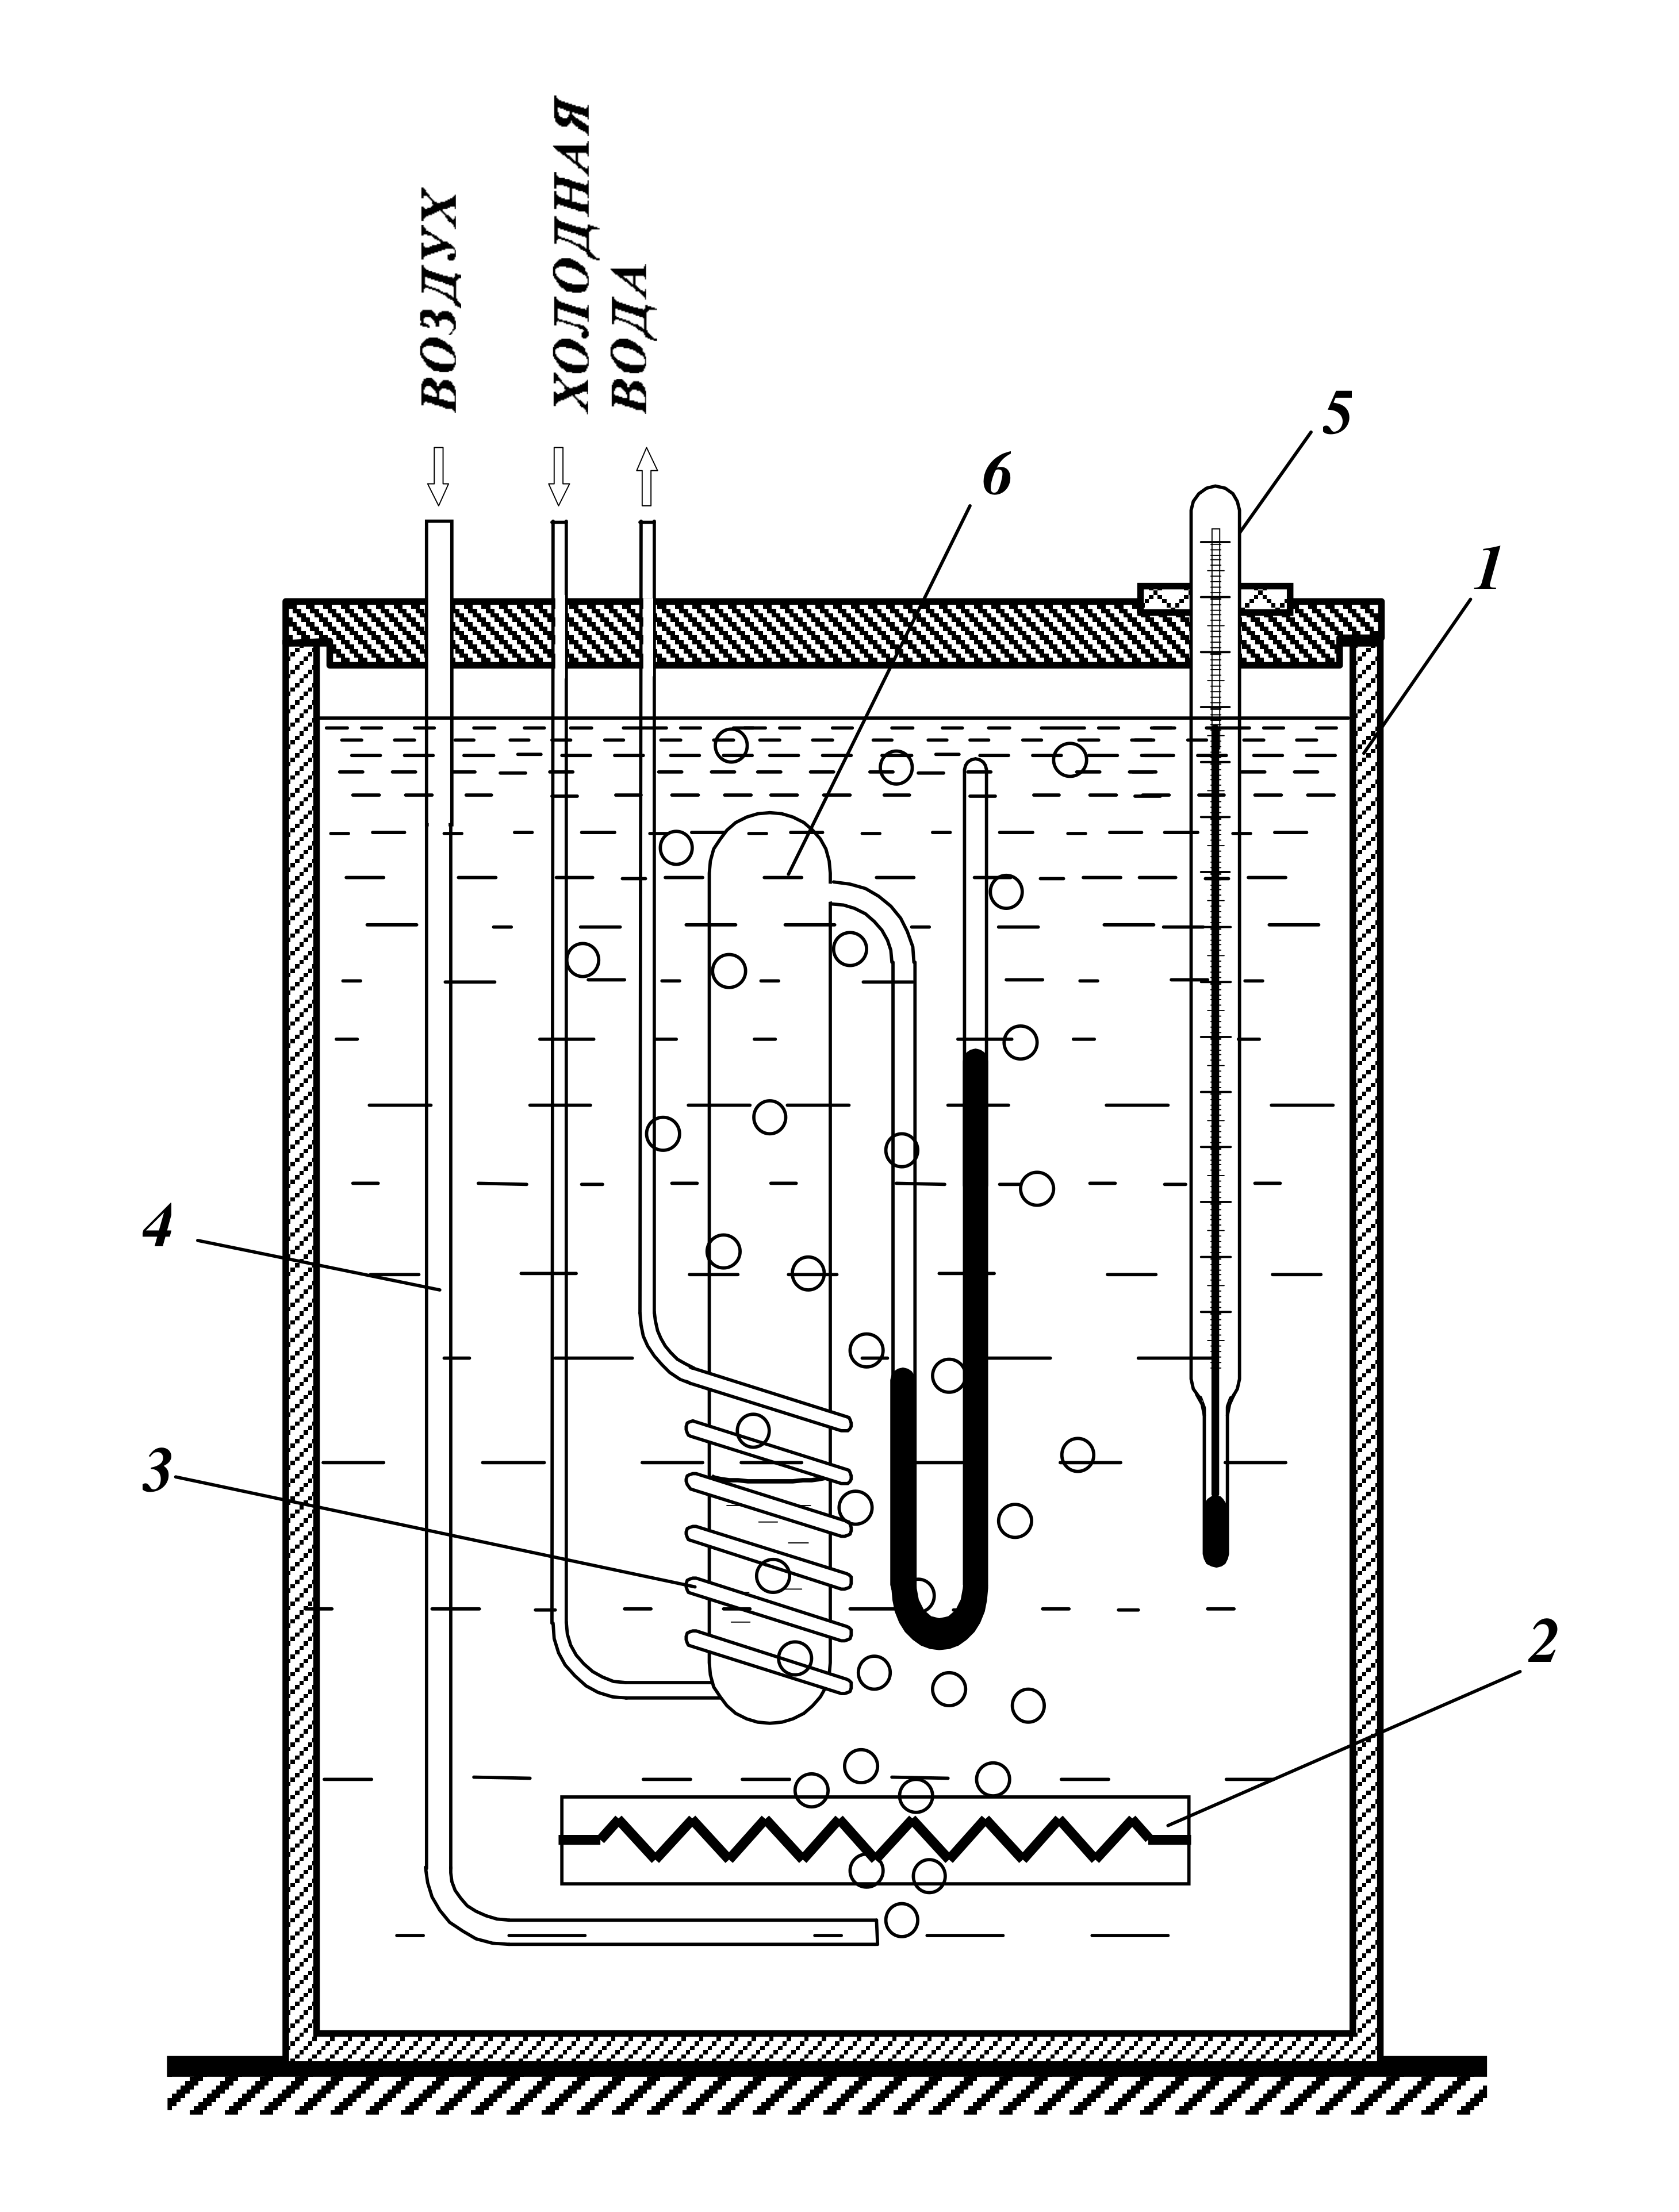
\includegraphics[width=0.5\textwidth]{setup.png}
\end{center}
\caption{Схема экспериментальной установки}
\label{fig:setup}
\end{figure}

\paragraph{Обозначения на рисунке \ref{fig:setup}:}

\begin{enumerate}
\renewcommand{\labelenumi}{\arabic{enumi} --}
\itemsep0em

\item Резервуар, играющий роль термостата.
\item Спираль подогревающая термостат электрическим током.
\item Змеевик по которому пропускается холодная вода для охлаждения термостата.
\item Трубка через которую в термостат подаётся воздух.
\item Термометр для измерения температуры термостата.
\item Запаянный прибор с исследуемой жидкостью.

\end{enumerate}

\paragraph{Погрешности установки:}
\begin{itemize}
\renewcommand{\labelitemi}{$\triangleright$}
\item Погрешность измерения температуры $\sigma_T = 0.1$ К
\item Погрешность измерения высоты $\sigma_h = 0.1$ мм
\end{itemize}

\subsection{Проведение эксперимента}

\begin{enumerate}
\itemsep0em

\item
Измерим разность уровней в ртутном U-образном манометре с помощью микроскопа и температуру по термометру.
\item
Включим термостат. Через каждый градус нагрева будем фиксировать температуру и давление, до 40-50 \degree C, либо до прохождения половины доступного времени.
\item
Проведём те же измерения при охлаждении жидкости. Следует установит воды, чтобы остывание проходило с тем же темпом, что и нагревание.
\item
Построим графики полученных данных в координатах $T$, $P$ и $1/T$, $\ln{P}$. 

\end{enumerate}

\subsection{Обработка результатов}

\paragraph{Полученные результаты.}
Копия листа с полученными результатами предоставлена в приложении. Найдём давление в каждый момент времени. Знаем что начальная высота правого столба $h_0 = 64.5$ мм, разница в высоте между ртутными столбами $ \Delta h_0 = 18 $ мм. Найдём давление в мм рт. ст. по формуле $ p = \Delta h_0 + 2(h - h_0) $, где $h$ -- измеренная высота правого столба. Переведём давление в мм рт. ст. в Па домножив значения на $133.32$. Полученные значения представлены в таблицах \ref{tab:data_up} и \ref{tab:data_down}.


\begin{table}[h]
\begin{center}
\begin{tabular}{|l|c|c|c|c|c|c|c|c|c|}
\hline 
$T$, К & 293 & 294 & 295 & 296 & 297 & 298 & 299 & 300 & 301 \\ 
\hline 
$P$, мм рт. ст. & 18.0 & 17.6 & 19.4 & 19.4 & 20.8 & 21.8 & 23.2 & 25.0 & 26.4 \\ 
\hline
$P$, Па & 2400 & 2346 & 2586 & 2586 & 2773 & 2906 & 3093 & 3333 & 3520 \\
\hline 
\hline
$T$, К & 302 & 303 & 304 & 305 & 306 & 307 & 308 & 309 & -- \\ 
\hline 
$P$, мм рт. ст. & 29.0 & 31.4 & 33.0 & 34.6 & 36.8 & 39.6 & 41.8 & 43.6 & -- \\ 
\hline
$P$, Па &  3866 & 4186 & 4400 & 4613 & 4906 & 5279 & 5573 & 5813 & -- \\
\hline 
\end{tabular} 
\end{center}
\caption{Измеренные значения давления при повышении температуры}
\label{tab:data_up}
\end{table}
	
\begin{table}[h]
\begin{center}
\begin{tabular}{|l|c|c|c|c|c|c|c|c|c|}
\hline 
$T$, К & 309 & 308 & 307 & 306 & 305 & 304 & 303 & 302 & 301 \\ 
\hline 
$P$, мм рт. ст. & 43.6 & 42.6 & 40.2 & 37.0 & 36.2 & 32.8 & 31.0 & 29.4 & 28.0 \\ 
\hline
$P$, Па & 5813 & 5679 & 5359 & 4933 & 4826 & 4373 & 4133 & 3920 & 3733 \\
\hline 
\hline
$T$, К & 300 & 299 & 298 & 297 & 296 & 295 & 294 & 293 & -- \\ 
\hline 
$P$, мм рт. ст. & 26.4 & 24.6 & 23.4 & 22.2 & 21.4 & 19.2 & 18.2 & 16.6 & -- \\ 
\hline 
$P$, Па & 3520 & 3280 & 3120 & 2960 & 2853 & 2560 & 2426 & 2213 & -- \\
\hline 
\end{tabular} 
\end{center}
\caption{Измеренные значения давления при понижении температуры}
\label{tab:data_down}
\end{table}

\paragraph{}
Далее для каждого значения $P$ найдём $\ln(P/P_0)$, где $P_0$ - значение давления при первом измерении при 20 \degree С. И также найдём $1/T$ и переведём в значение в $\text{К}^{-1} \cdot 10^3$. Эти значения приведены в таблицах \ref{tab:graph_up} и \ref{tab:graph_down}, они будут использоваться для построения графика.

\begin{table}[h]
\begin{center}
\begin{tabular}{|l|c|c|c|c|c|c|c|c|c|}
\hline 
$1/T, \; \text{K}^{-1} \cdot 10^3$ & 3.413 & 3.401 & 3.39 & 3.378 & 3.367 & 3.356 & 3.344 & 3.333 & 3.322 \\ 
\hline 
$\ln(P/P_0)$ & 0.0 & -0.022 & 0.075 & 0.075 & 0.145 & 0.192 & 0.254 & 0.329 & 0.383 \\
\hline 
\hline
$1/T, \; \text{K}^{-1} \cdot 10^3$ &  3.311 & 3.3 & 3.289 & 3.279 & 3.268 & 3.257 & 3.247 & 3.236 & -- \\ 
\hline 
$\ln(P/P_0)$ &  0.477 & 0.556 & 0.606 & 0.653 & 0.715 & 0.788 & 0.843 & 0.885 & -- \\
\hline 
\end{tabular} 
\end{center}
\caption{Точки для построения логарифмического графика для повышения температуры}
\label{tab:graph_up}
\end{table}

\begin{table}[h]
\begin{center}
\begin{tabular}{|l|c|c|c|c|c|c|c|c|c|}
\hline 
$1/T, \; \text{K}^{-1} \cdot 10^3$ & 3.236 & 3.247 & 3.257 & 3.268 & 3.279 & 3.289 & 3.3 & 3.311 & 3.322 \\ 
\hline 
$\ln(P/P_0)$ & 0.885 & 0.861 & 0.803 & 0.721 & 0.699 & 0.6 & 0.544 & 0.491 & 0.442 \\
\hline 
\hline
$1/T, \; \text{K}^{-1} \cdot 10^3$ & 3.333 & 3.344 & 3.356 & 3.367 & 3.378 & 3.39 & 3.401 & 3.413 & -- \\ 
\hline 
$\ln(P/P_0)$ & 0.383 & 0.312 & 0.262 & 0.21 & 0.173 & 0.065 & 0.011 & -0.081 & -- \\
\hline 
\end{tabular} 
\end{center}
\caption{Точки для построения логарифмического графика для понижения температуры}
\label{tab:graph_down}
\end{table}

\paragraph{Нахождение наилучшей прямой.}
Для графиков зависимости $ P(T) $ и $ \ln{(P/P_0)}(1/T )$ найдём наилучшую прямую по методу наименьших квадратов. Метод наименьших квадратов для построения прямой $ y = A + B x $:
\begin{equation}
B = \frac{\langle xy \rangle - \langle x \rangle \langle y \rangle}{\langle x^2 \rangle - \langle x \rangle ^ 2}, \;\;
A = \langle y \rangle - B \langle x \rangle . \label{lsf}
\end{equation}
Погрешности коэффициентов $a$ и $b$ находятся по формулам:
\begin{equation}
\sigma_B \approx \frac{1}{\sqrt{N}}\sqrt{\frac{\langle y^2 \rangle - \langle y \rangle ^ 2}{\langle x^2 \rangle - \langle x \rangle ^ 2} - B^2}, \;\;
\sigma_A = \sigma_B \sqrt{\langle x^2 \rangle - \langle x \rangle ^ 2}. \label{lsfvar}
\end{equation}

\subsection{Построение графиков}

\paragraph{График $\textbf{P(T)}$}
Найдём наилучшую прямую подставив в (\ref{lsf}) и (\ref{lsfvar}) вместо $x$ и $y$ значения $T$ и $P$ из таблиц \ref{tab:data_up} и \ref{tab:data_down}. Получаем:

\begin{enumerate}
\item При повышении температуры:
\begin{center}
\begin{tabular}{|c|c|}
\hline 
$\langle x \rangle$ & 301.0 \\ 
\hline 
$\langle y \rangle$ & 3775.3 \\ 
\hline 
$\langle x^2 \rangle$ & 90625 \\ 
\hline 
$\langle y^2 \rangle$ & 15514052 \\ 
\hline 
$\langle xy \rangle$ & 1141791 \\ 
\hline 
$N$ & 17 \\ 
\hline 
\end{tabular} 
\end{center}

Получаем:
\[
B = \frac{1141791 - 301 \cdot 3775}{90625 - 301^2} \approx 226 \text{Па/К}, \;\;\;
A = 3775 - 226 \cdot 301 \approx -64248 \text{Па}.
\]
Считаем погрешность:
\[
\sigma_B = \frac{1}{\sqrt{17}} \sqrt{\frac{15514052 - 3775^2}{90625 - 301^2} - 226^2} \approx 9 \text{Па/К}, \;\;\; \sigma_A = 9 \sqrt{90625 - 301^2} \approx 46 \text{Па}.
\]

\item При понижении температуры:

\begin{center}
\begin{tabular}{|c|c|}
\hline 
$\langle x \rangle$ & 301 \\ 
\hline 
$\langle y \rangle$ & 3864 \\ 
\hline 
$\langle x^2 \rangle$ & 90625 \\ 
\hline 
$\langle y^2 \rangle$ & 16176968 \\ 
\hline 
$\langle xy \rangle$ & 1168695 \\ 
\hline 
$N$ & 17 \\ 
\hline 
\end{tabular} 
\end{center}

Получаем:
\[
B = \frac{1168695 - 301 \cdot 3864}{90625 - 301^2} \approx 226 \text{Па/К}, \;\;\;
A = 3864 - 226 \cdot 301 \approx -64079 \text{Па}.
\]
Считаем погрешность:
\[
\sigma_B = \frac{1}{\sqrt{17}} \sqrt{\frac{16176968 - 3864^2}{90625 - 301^2} - 226^2} \approx 7 \text{Па/К}, \;\;\; \sigma_A = 7 \sqrt{90625 - 301^2} \approx 33 \text{Па}.
\]

\item По всем точкам

\begin{center}
\begin{tabular}{|c|c|}
\hline 
$\langle x \rangle$ & 301 \\ 
\hline 
$\langle y \rangle$ & 3820 \\ 
\hline 
$\langle x^2 \rangle$ & 90625 \\ 
\hline 
$\langle y^2 \rangle$ & 15845510 \\ 
\hline 
$\langle xy \rangle$ & 1155243 \\ 
\hline 
$N$ & 34 \\ 
\hline 
\end{tabular} 
\end{center}

Получаем:
\[
B = \frac{1155243 - 301 \cdot 3820}{90625 - 301^2} \approx 226 \text{Па/К}, \;\;\;
A = 3820 - 226 \cdot 301 \approx -64164 \text{Па}.
\]
Считаем погрешность:
\[
\sigma_B = \frac{1}{\sqrt{34}} \sqrt{\frac{15845510 - 3820^2}{90625 - 301^2} - 226^2} \approx 6 \text{Па/К}, \;\;\; \sigma_A = 6 \sqrt{90625 - 301^2} \approx 29 \text{Па}.
\]

\end{enumerate}

По полученным значениям строим график (рис. \ref{fig:graph1}).

\begin{figure}
\begin{center}
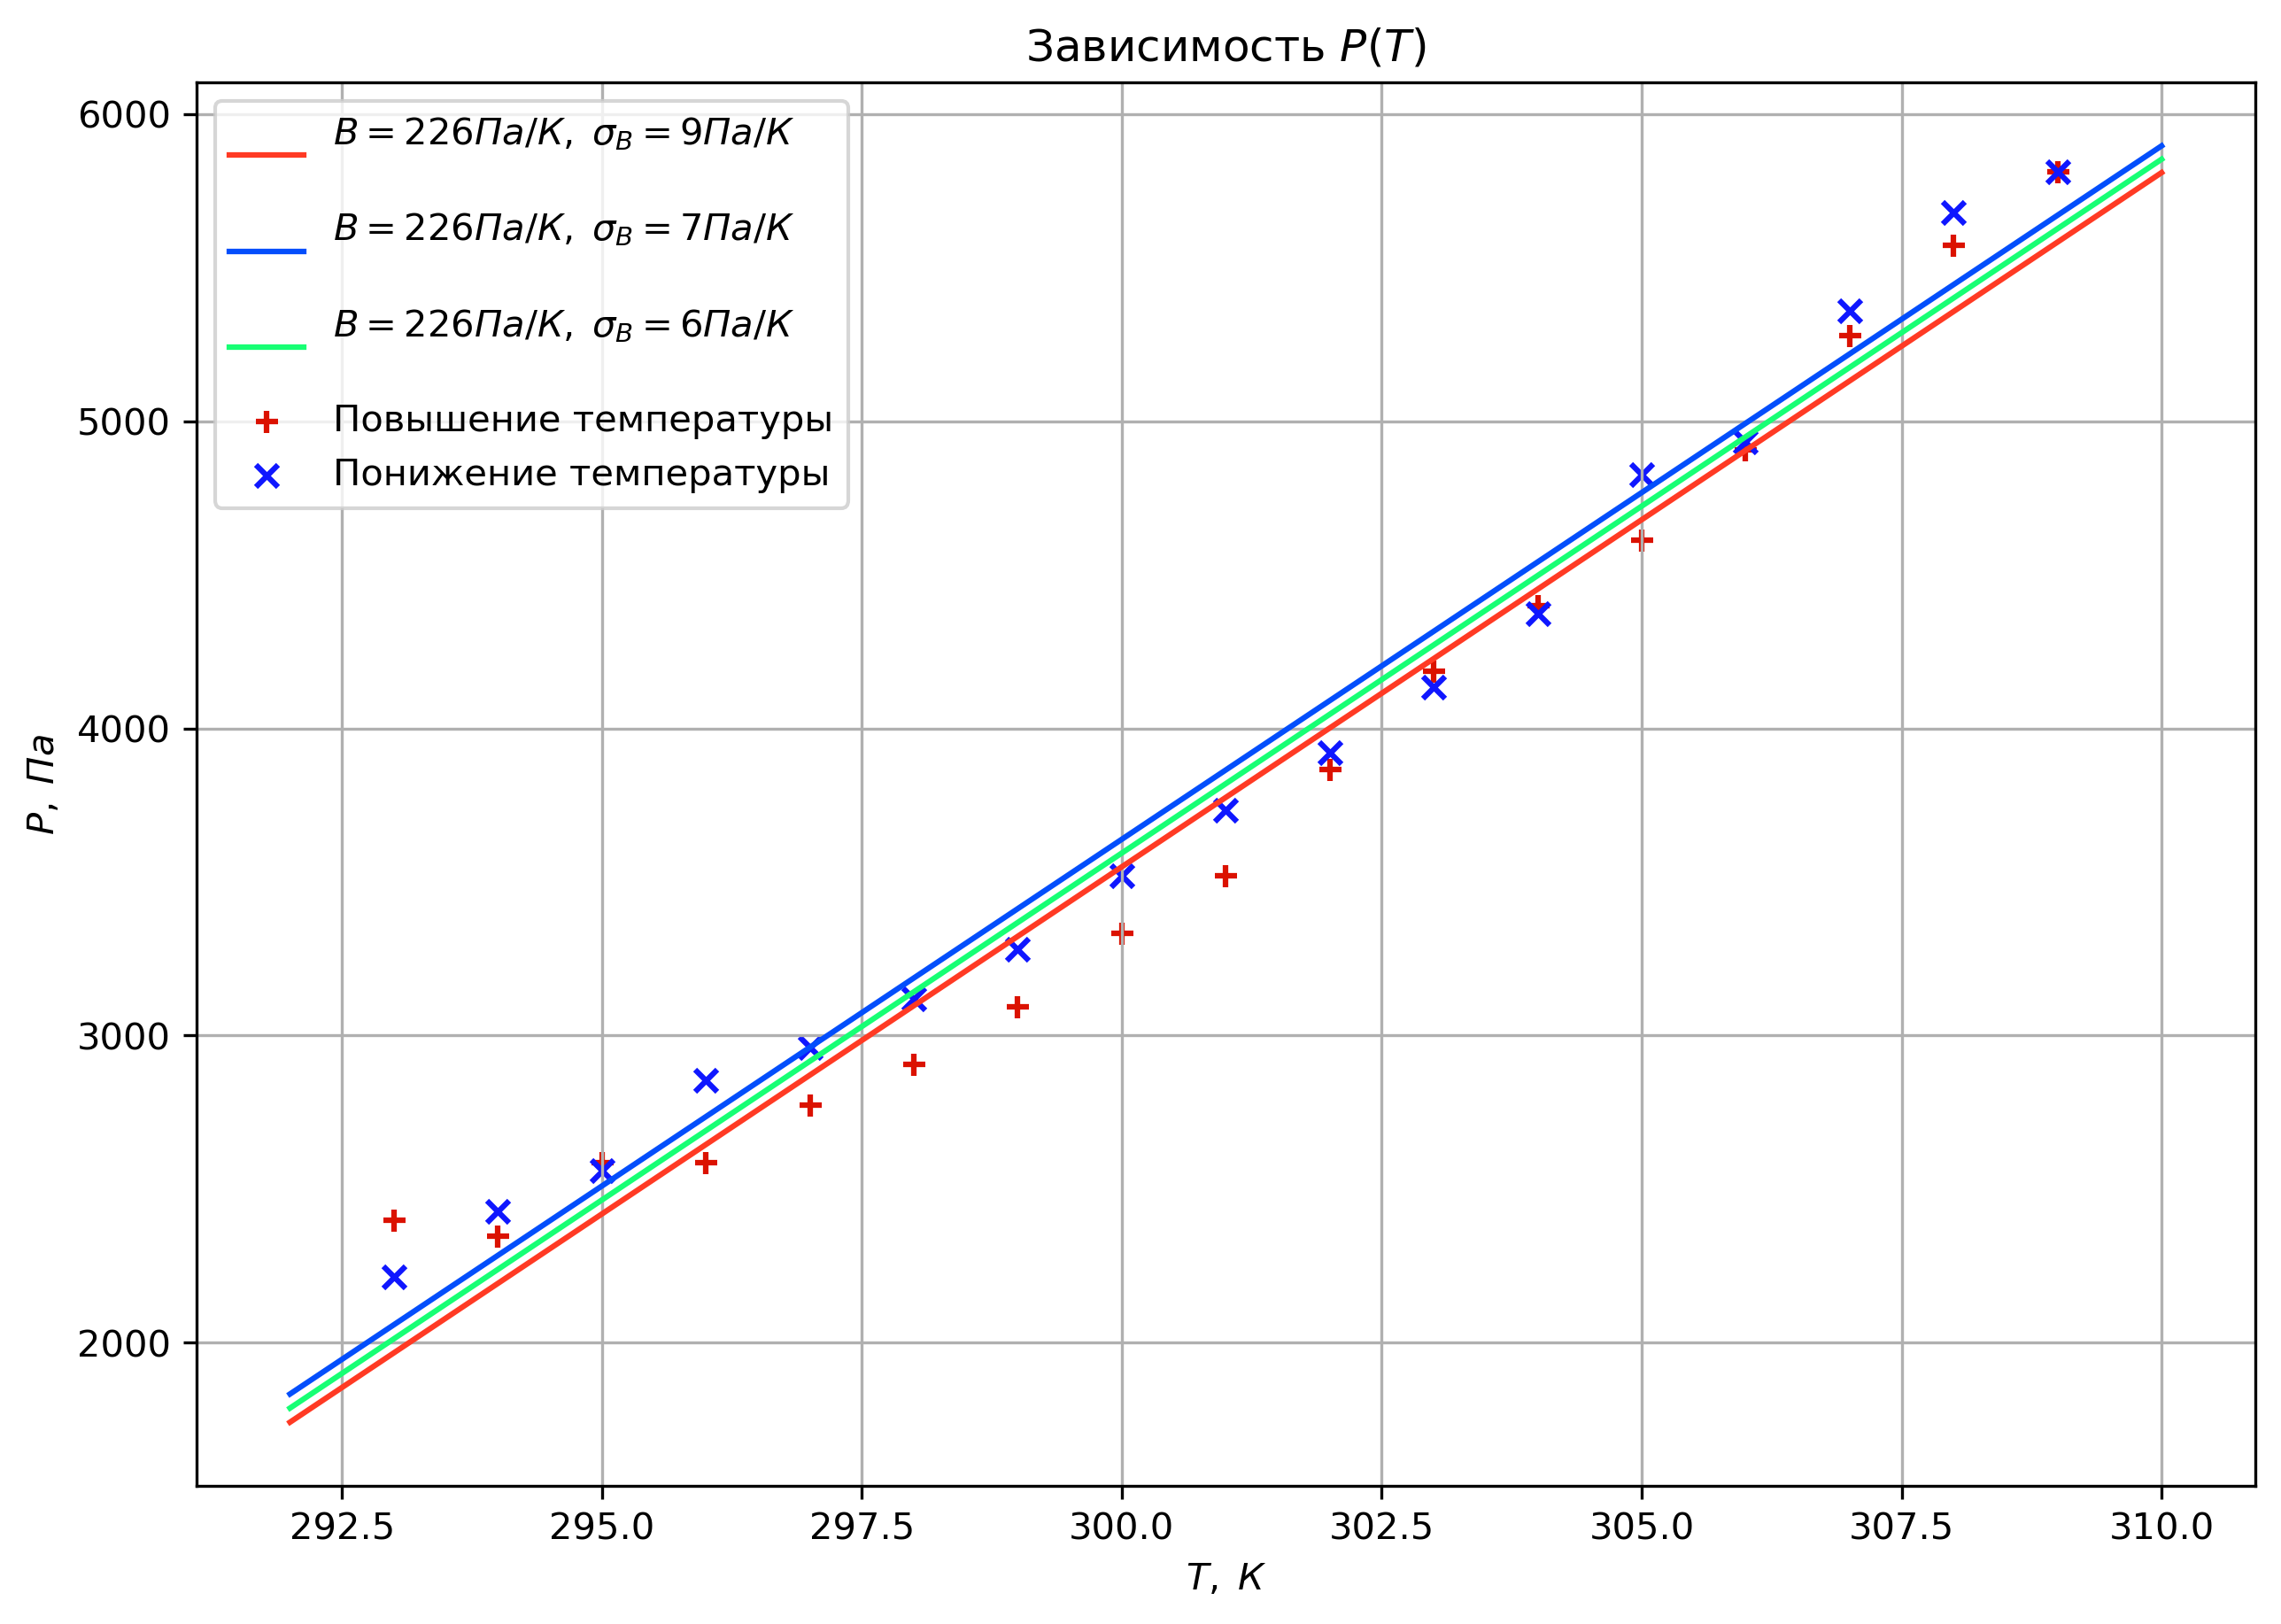
\includegraphics[width=\textwidth]{graph1.png}
\end{center}
\caption{Первый график}
\label{fig:graph1}
\end{figure}

\paragraph{График $ \ln{P/P_0} (1/T) $}
Найдём наилучшую прямую подставив в (\ref{lsf}) и (\ref{lsfvar}) вместо $ x $ и $ y $ значения $ 1/T $ и $ \ln{(P/P_0)} $ из таблиц \ref{tab:graph_up} и \ref{tab:graph_down}. Получаем:

\begin{enumerate}
\item При повышении температуры:
\begin{center}
\begin{tabular}{|c|c|}
\hline 
$\langle x \rangle$ & 3.323 \\ 
\hline 
$\langle y \rangle$ & 0.409 \\ 
\hline 
$\langle x^2 \rangle$ & 11.046 \\ 
\hline 
$\langle y^2 \rangle$ & 0.256 \\ 
\hline 
$\langle xy \rangle$ & 1.343 \\ 
\hline 
$N$ & 17 \\ 
\hline 
\end{tabular} 
\end{center}

Получаем:
\[
B = \frac{1.343 - 3.323 \cdot 0.409}{11.046 - 3.323^2} \approx -5.46 \text{К}\cdot 10^3, \;\;\;
A = 0.409 + 5.46 \cdot 3.323 \approx 18.57.
\]
Считаем погрешность:
\[
\sigma_B = \frac{1}{\sqrt{17}} \sqrt{\frac{0.256 - 0.409^2}{11.046 - 3.323^2} - 5.46^2} \approx 0.13 \text{К}\cdot 10^3, \;\;\; \sigma_A = 0.13 \sqrt{11.046 - 3.323^2} \approx 0.01.
\]

\item При понижении температуры:

\begin{center}
\begin{tabular}{|c|c|}
\hline 
$\langle x \rangle$ & 3.323 \\ 
\hline 
$\langle y \rangle$ & 0.434 \\ 
\hline 
$\langle x^2 \rangle$ & 11.046 \\ 
\hline 
$\langle y^2 \rangle$ & 0.275 \\ 
\hline 
$\langle xy \rangle$ & 1.426 \\ 
\hline 
$N$ & 17 \\ 
\hline 
\end{tabular} 
\end{center}

Получаем:
\[
B = \frac{1.426 - 3.323 \cdot 0.434}{11.046 - 3.323^2} \approx -5.41 \text{К}\cdot 10^3, \;\;\;
A = 0.434 + 5.41 \cdot 3.323 \approx 18.426.
\]
Считаем погрешность:
\[
\sigma_B = \frac{1}{\sqrt{17}} \sqrt{\frac{0.275 - 0.434^2}{11.046 - 3.323^2} - 5.46^2} \approx 0.07 \text{К}\cdot 10^3, \;\;\; \sigma_A = 0.07 \sqrt{11.046 - 3.323^2} \approx 0.004.
\]

\item По всем точкам

\begin{center}
\begin{tabular}{|c|c|}
\hline 
$\langle x \rangle$ & 3.323 \\ 
\hline 
$\langle y \rangle$ & 0.422 \\ 
\hline 
$\langle x^2 \rangle$ & 11.046 \\ 
\hline 
$\langle y^2 \rangle$ & 0.265 \\ 
\hline 
$\langle xy \rangle$ & 1.385 \\ 
\hline 
$N$ & 34 \\ 
\hline 
\end{tabular} 
\end{center}

Получаем:
\[
B = \frac{1.385 - 3.323 \cdot 0.422}{11.046 - 3.323^2} \approx -5.41 \text{К}\cdot 10^3, \;\;\;
A = 0.422 + 5.41 \cdot 3.323 \approx 18.426.
\]
Считаем погрешность:
\[
\sigma_B = \frac{1}{\sqrt{17}} \sqrt{\frac{0.265 - 0.422^2}{11.046 - 3.323^2} - 5.46^2} \approx 0.09 \text{К}\cdot 10^3, \;\;\; \sigma_A = 0.09 \sqrt{11.046 - 3.323^2} \approx 0.005.
\]


\end{enumerate}

По полученным значениям строим график (рис. \ref{fig:graph2}).

\begin{figure}
\begin{center}
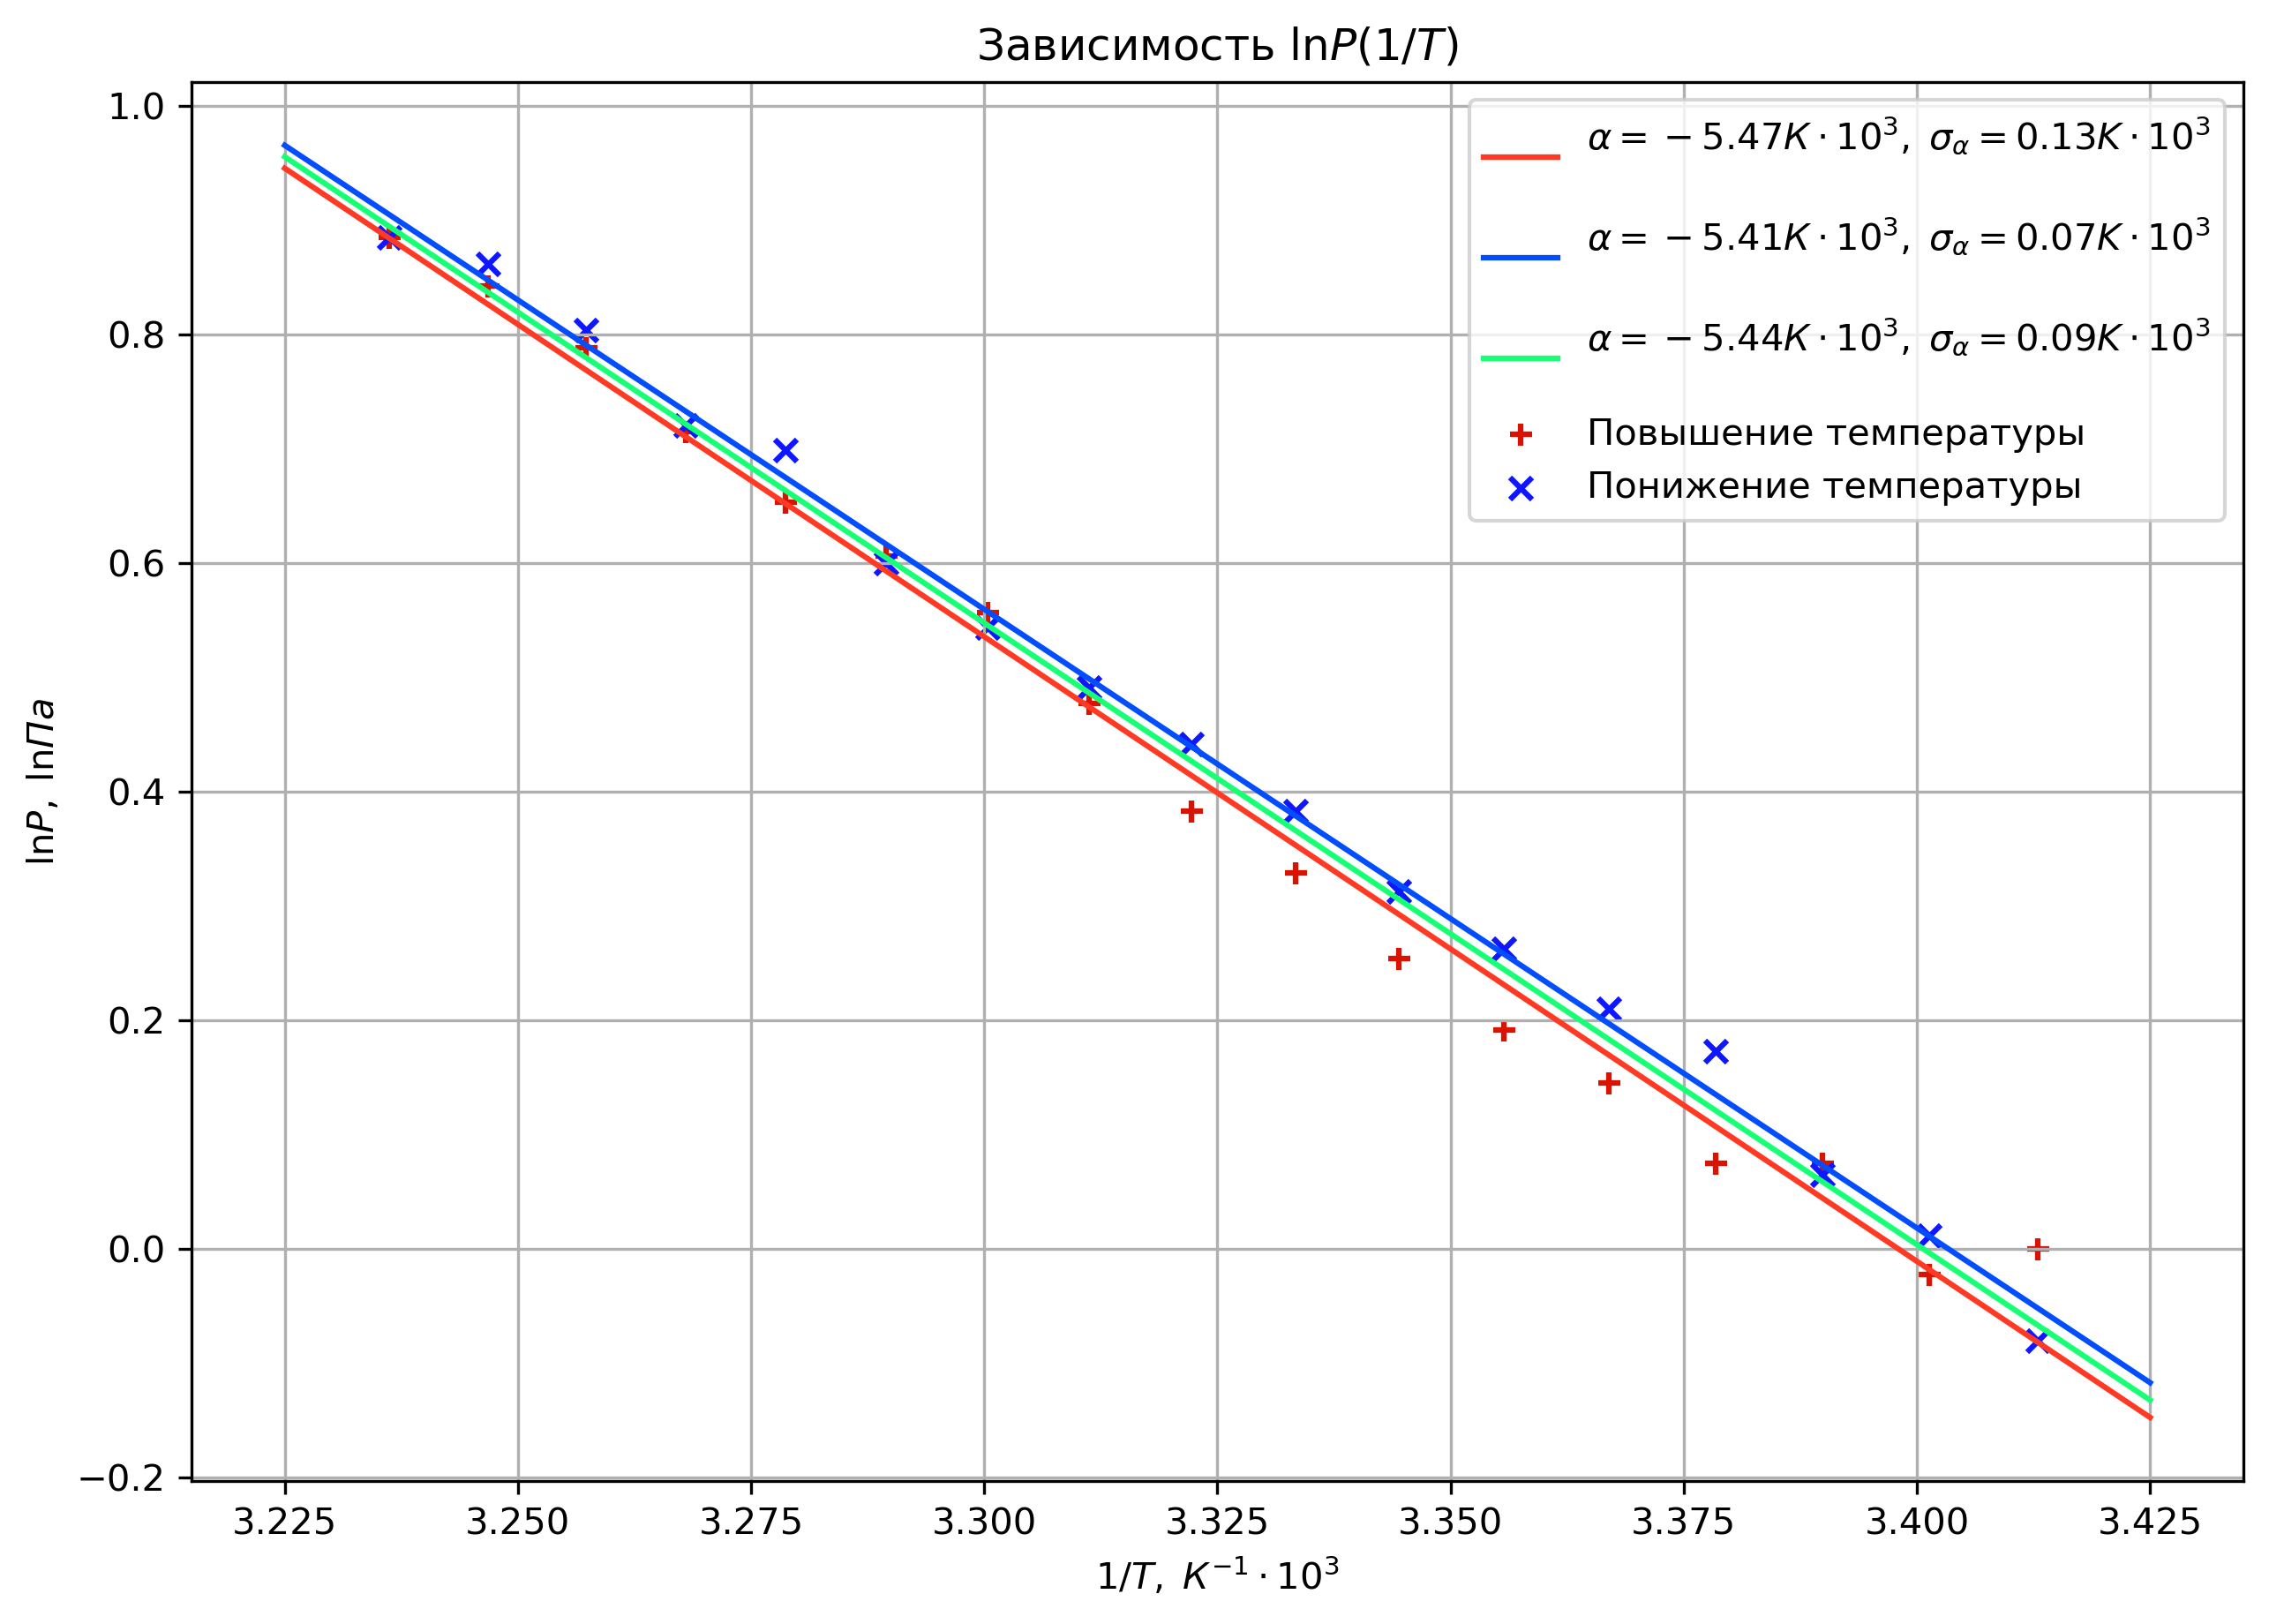
\includegraphics[width=\textwidth]{graph2.png}
\end{center}
\caption{Второй	 график}
\label{fig:graph2}
\end{figure}

\subsection{Расчёт конечных значений}

По полученным данным рассчитаем $L$ для углекислого газа.

В первом случае рассчитаем $L$ по данным полученным из первого графика. Возьмём значения с наименьшей погрешностью, то есть: $B = 226$ Па/К $\sigma_B = 6$ Па/К. Подставим в формулу \ref{eq:capacity} $B$ вместо $\frac{dP}{dT}$, возьмём $T = \langle T \rangle = 301$ К, на первом графике найдём значение $P$ соответствующее точке по $T = 301$ К по зелёной прямой, получим $P = 3820$ Па. Подставим значения:
\[
L = \frac{RT^2}{P} B = \frac{R \cdot 301^2}{3820} \cdot 226 \approx 44500 \frac{\text{Дж}}{\text{моль}}.
\]
Рассчитаем погрешность по формуле:
\[
\sigma_L = L 
\sqrt{4 \left(\frac{\sigma_T}{T} \right)^2 + 
\left(\frac{\sigma_P}{P} \right)^2 + 
\left(\frac{\sigma_B}{B} \right)^2} = 44500 \cdot \sqrt{4 
\left(\frac{0.1}{301}\right)^2 + \left(\frac{13}{3820}\right)^2 + 
\left(\frac{6}{226} \right)^2} \approx 1200 \frac{\text{Дж}}{\text{моль}}.
\]

Во втором случае рассчитаем $L$ по данным полученным из второго графика. Возьмём значения с наименьшей погрешностью, то есть: $B = -5.41 \cdot 10^3 $ К $\sigma_B = 0.07 \cdot 10^3$ К. Подставим в правую часть формулы \ref{eq:capacity} значение $B$ вместо $\frac{d(\ln(P)}{d(1/T)} $:
\[
L = - R \cdot B = 8.314 \cdot 5.41 \cdot 10^3 \approx 45200 \frac{\text{Дж}}{\text{моль}}.
\]
Рассчитаем погрешность по формуле:
\[
\sigma_L = L \frac{\sigma_B}{B} = 45200 \cdot \frac{0.07}{5.41} \approx 700 \frac{\text{Дж}}{\text{моль}}.
\]
Далее перейдём к выводам.

\section{Выводы}

\begin{enumerate}
\itemsep0em

\item Полученные в работе значения для молярной теплоёмкости $L$: $L_1 = 44.5 \pm 1.2 \; \frac{\text{кДж}}{\text{моль}} \; (\varepsilon_L = 3\%)$, $L_2 = 45.2 \pm 0.7 \; \frac{\text{кДж}}{\text{моль}} \; (\varepsilon_L = 2\%)$.

\item Видим, что построение графика в логарифмических координатах помогло добиться более точных значений. 

\item Сравнивая полученные значения для $L$ с табличным $L = 40.68 \; \frac{\text{кДж}}{\text{моль}}$, видим, что полученные данные не совпадают с табличными. Это можно связать с низким давлением в системе.

\end{enumerate}

\section{Приложение}

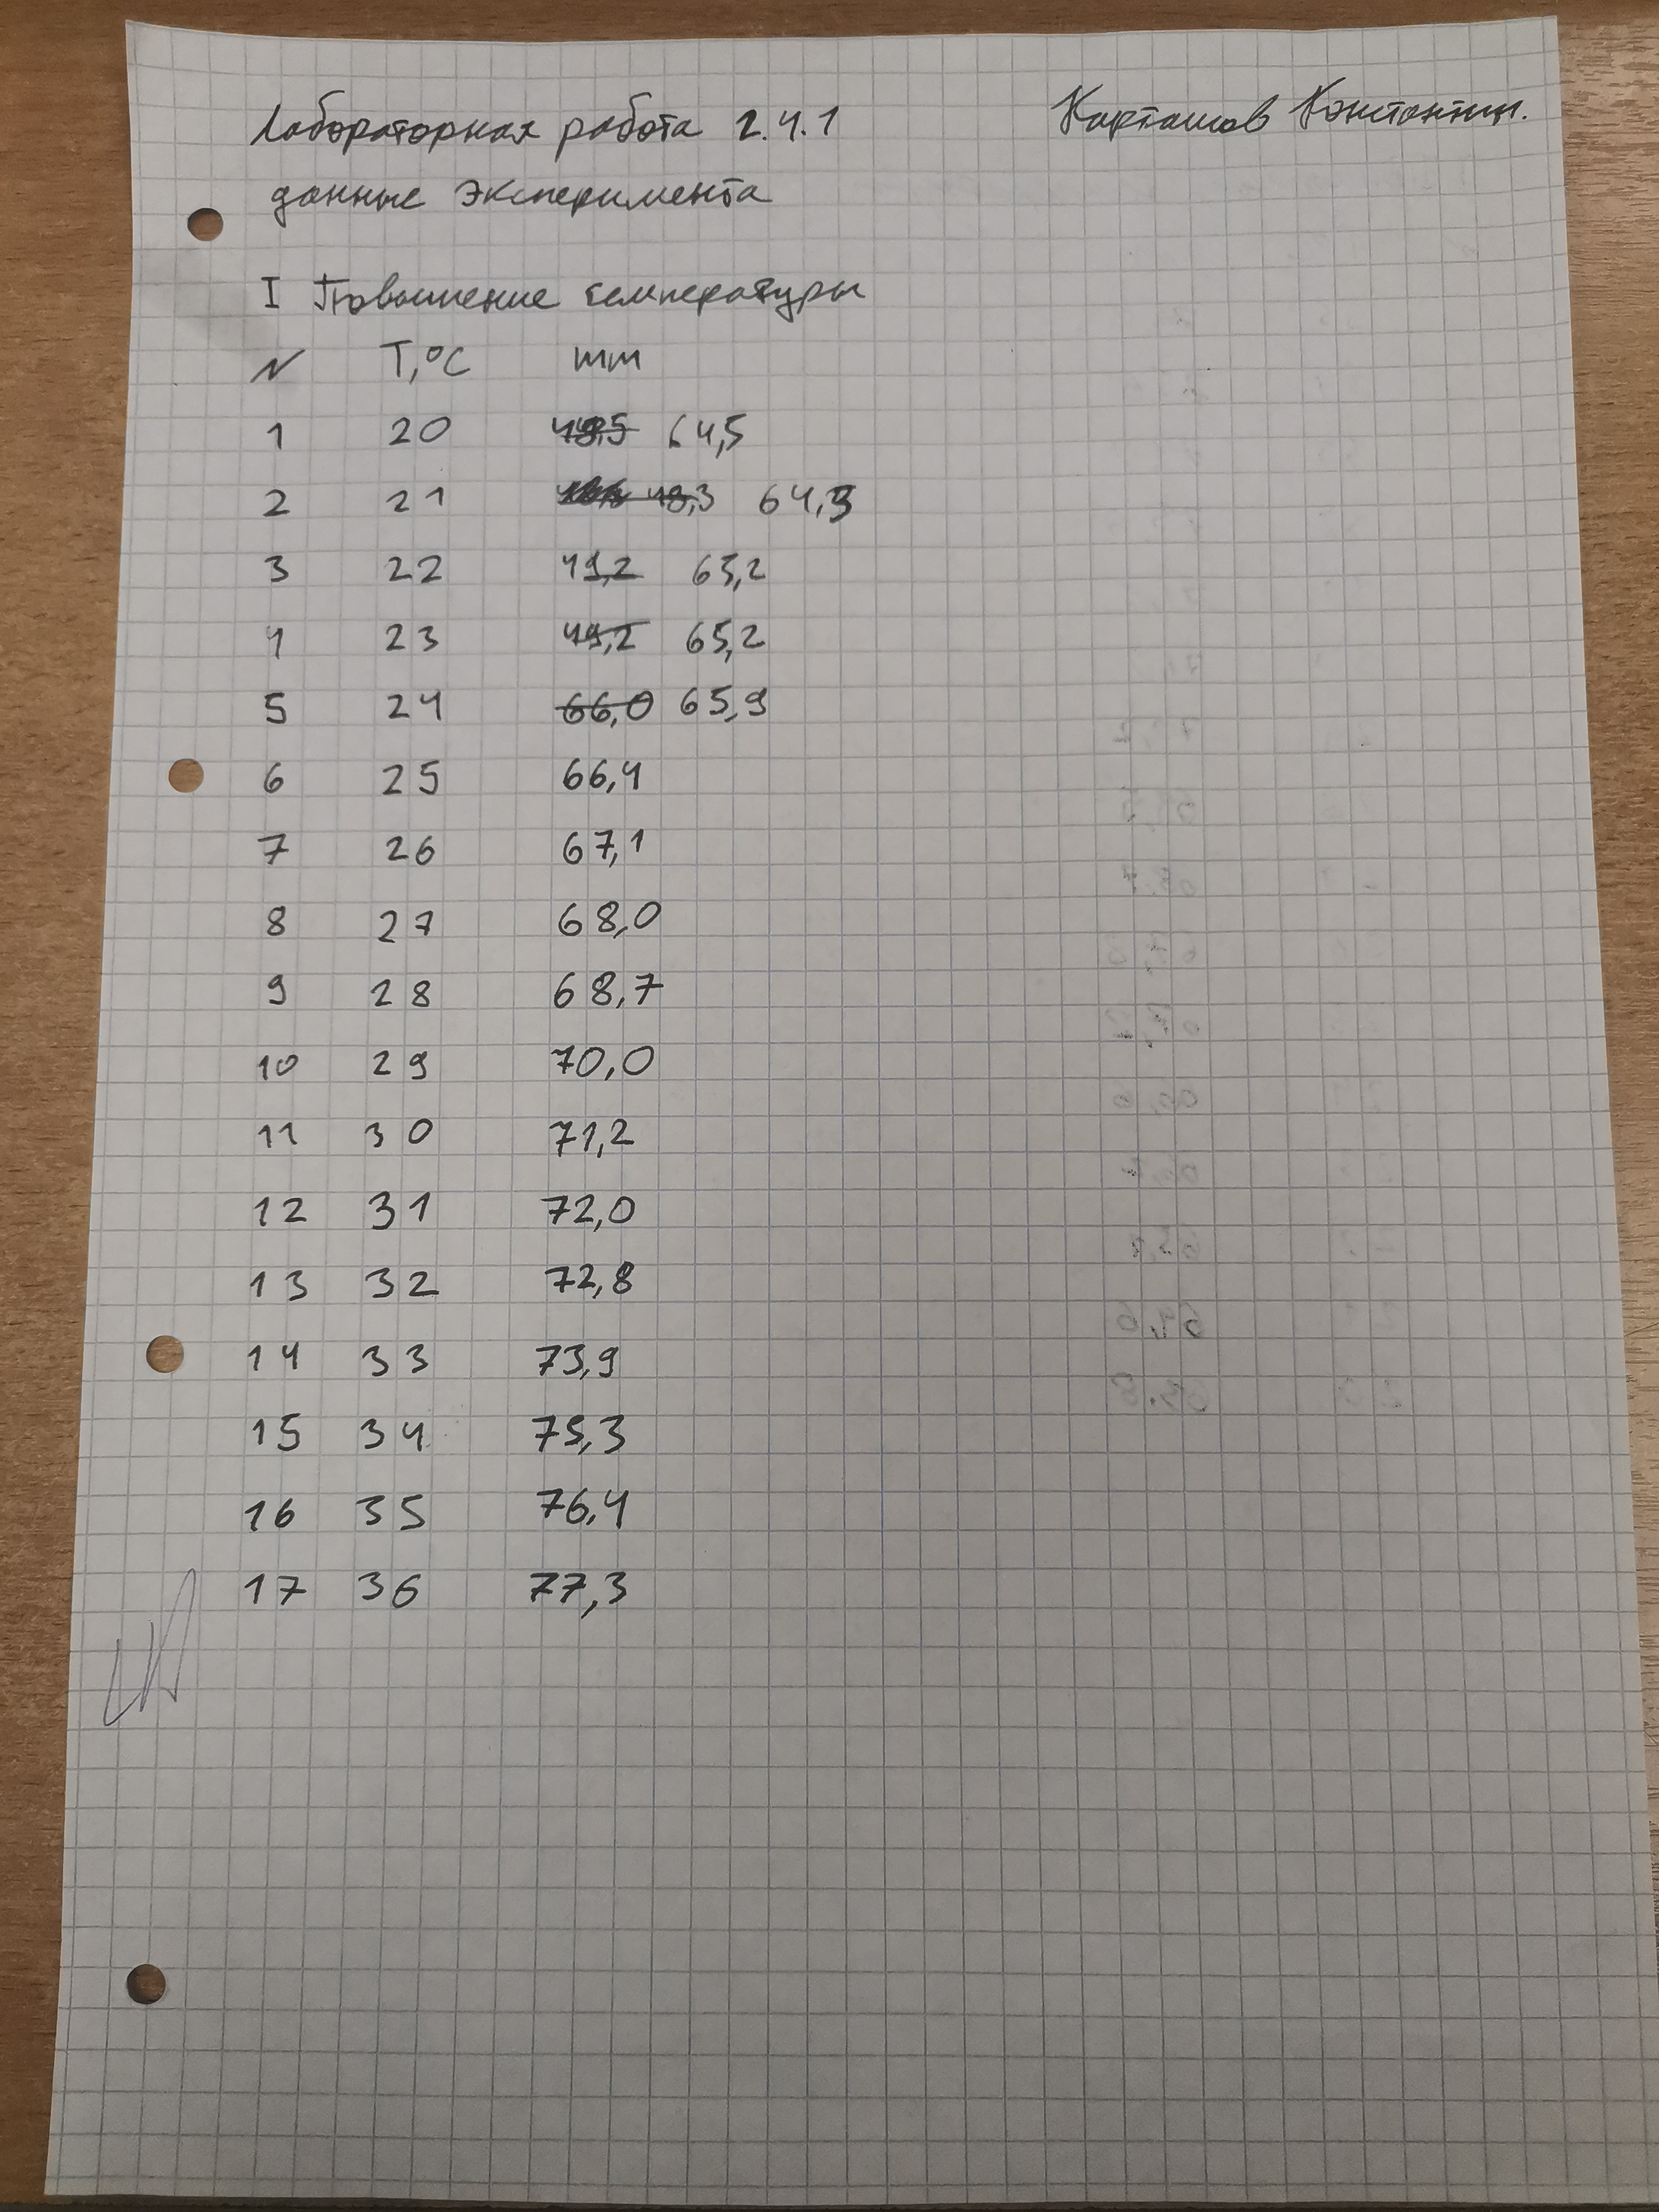
\includegraphics[width=1\textwidth]{page_1.jpg}

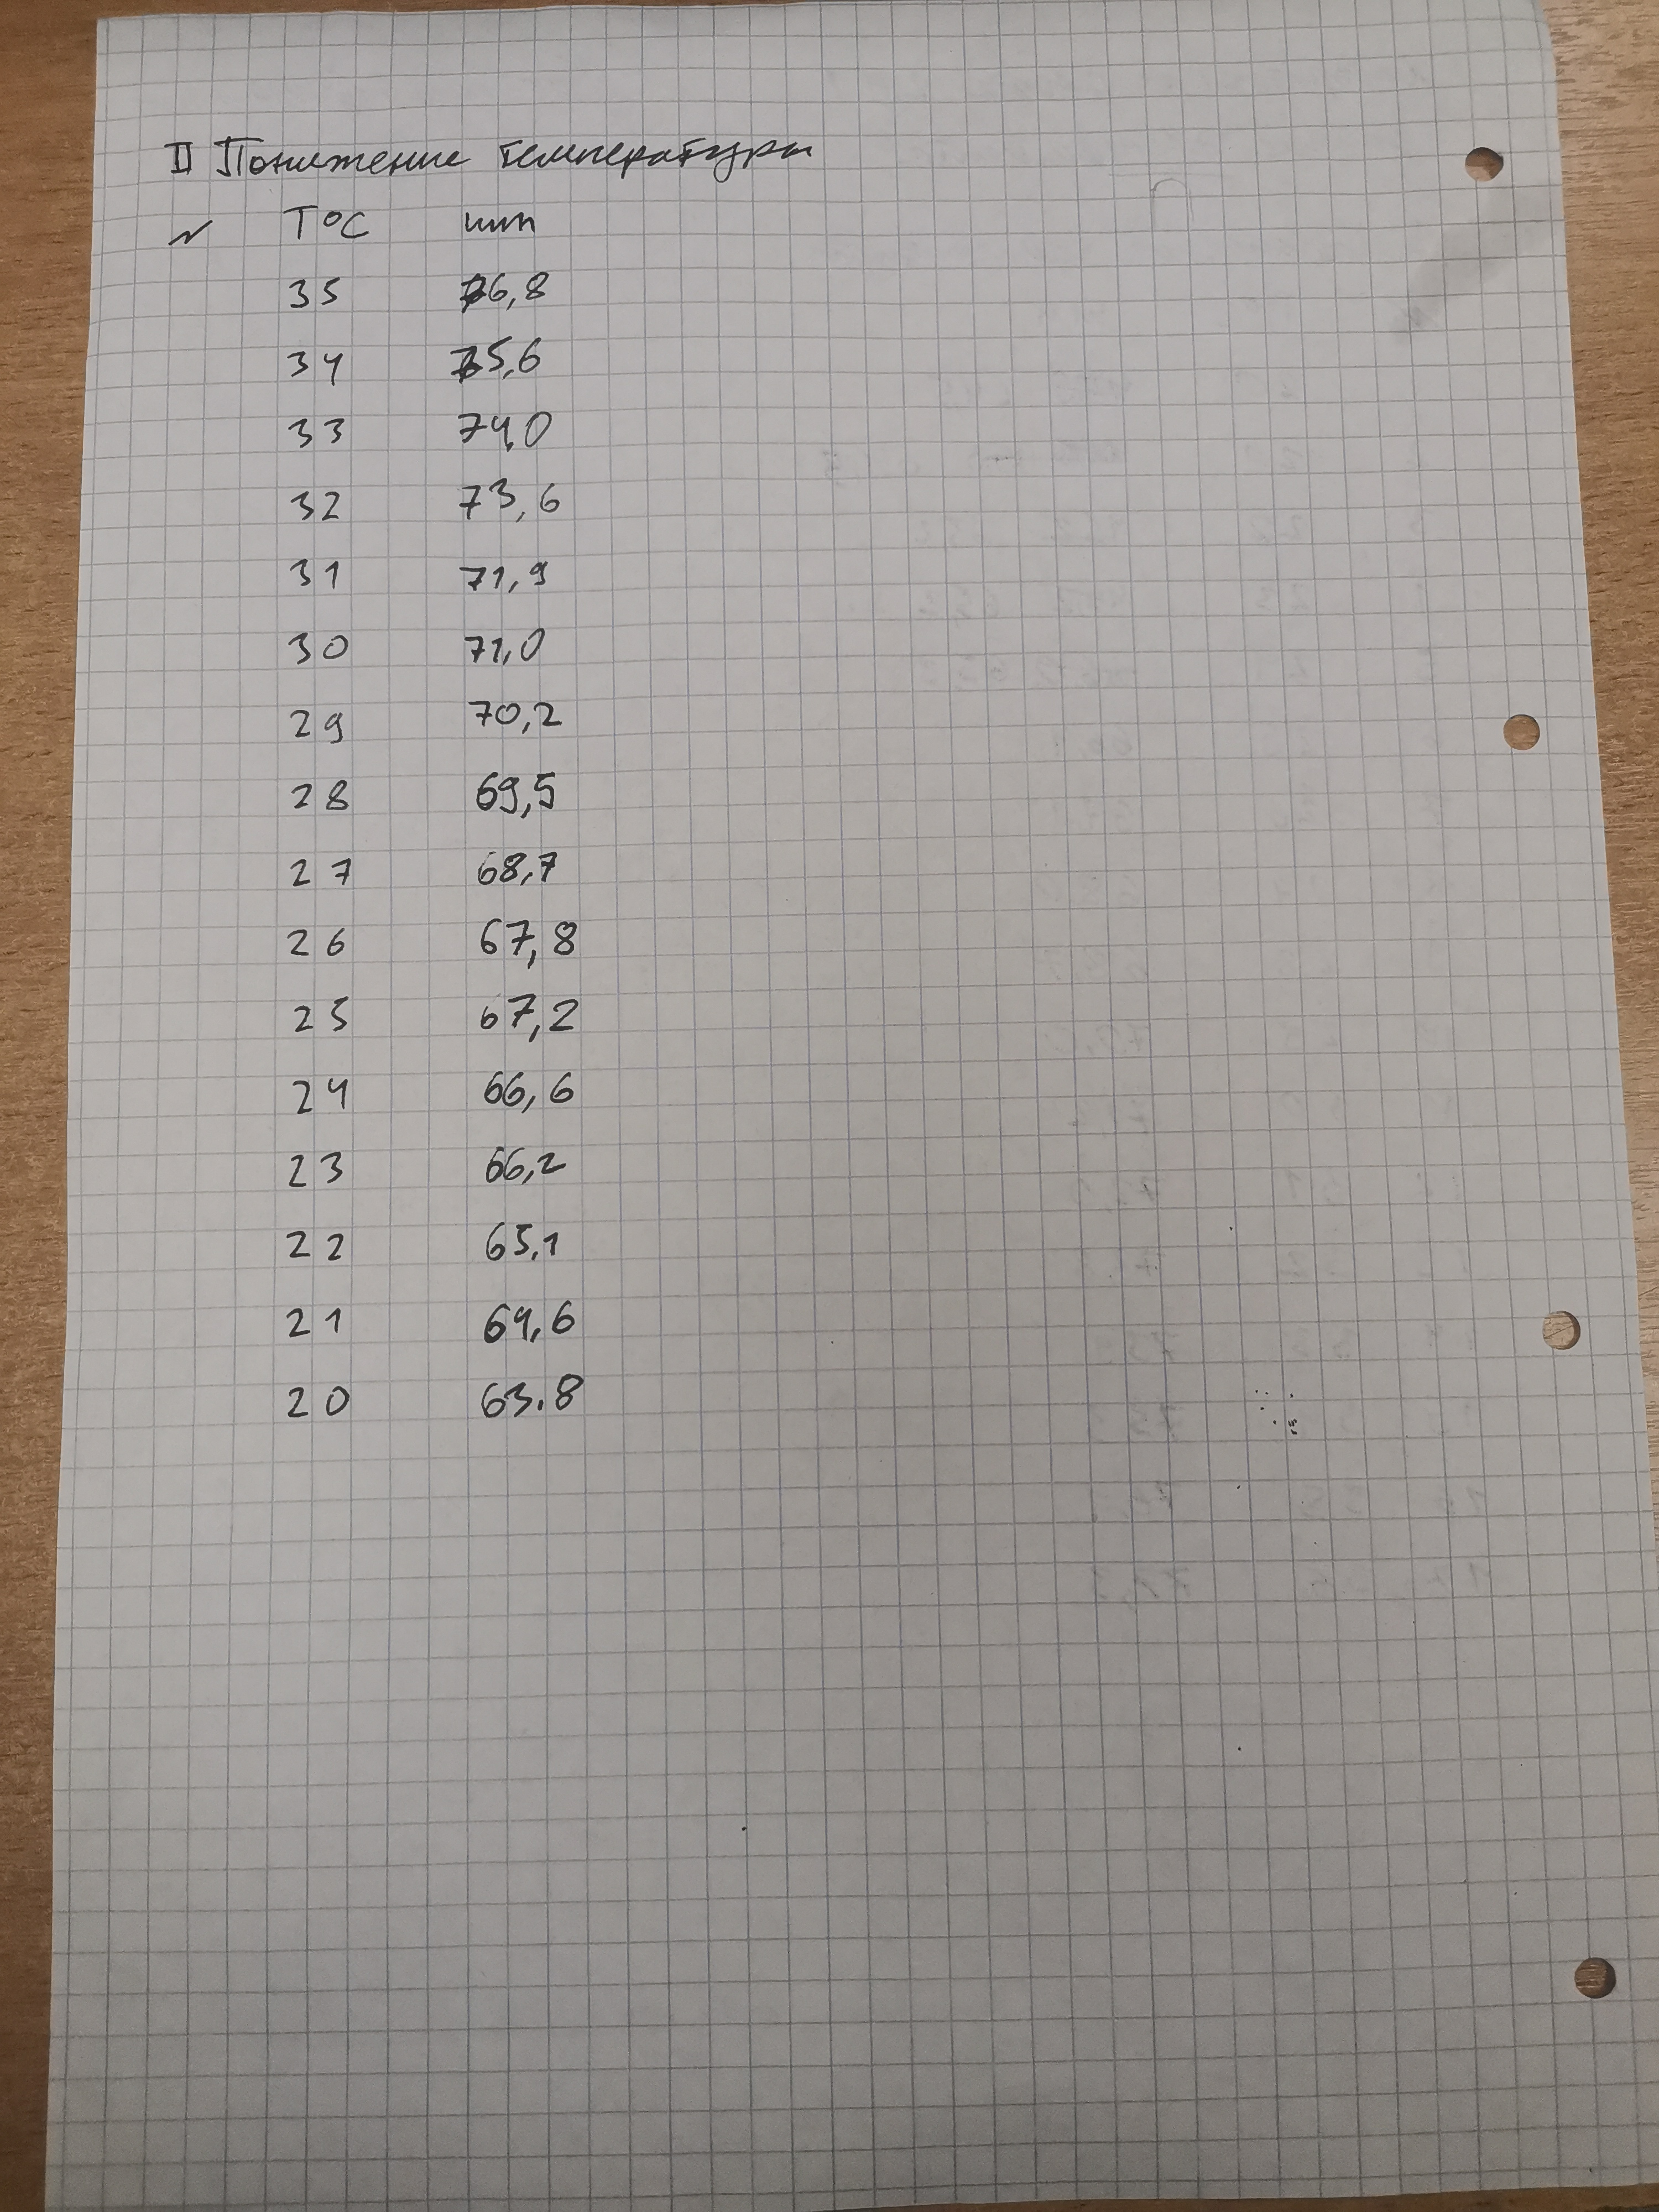
\includegraphics[width=1\textwidth]{page_2.jpg}

\end{document}


